\chapter{Modeling Stateful Protocols}
\label{ch:state}

\index{stateful protocols}
The {\cpsa} tool has the ability to also model stateful protocols:
that is, protocols in which participants interact through messages but
also with stateful devices the attacker is not assumed to have direct
control of.

\section{The Envelope Protocol}
\label{sec:envelope}

\index{envelope protocol}
We use Mark Ryan's Envelope Protocol~\cite{ArapinisEtAl2011} as a
concrete example throughout the chapter. The protocol leverages
cryptographic mechanisms supported by a Trusted Platform Modeul (TPM)
to allow one party to package a secret such that another party can
either reveal the secret or prove the secret never was and never will
be revealed, but not both.

The plight of a teenager motivates the protocol.  The teenager is
going out for the night, and her parents want to know her destination
in case of emergency.  Chafing at the loss of privacy, she agrees to
the following protocol.  Before leaving for the night, she writes her
destination on a piece of paper and seals the note in an envelope.
Upon her return, the parents can prove the secret was never revealed
by returning the envelope unopened. Alternatively, they can open the
envelope to learn her destination.

The parents would like to learn their daughter's destination while
still pretending that they have respected her privacy. The parents are
thus the adversary.  The goal of the protocol is to prevent this
deception.

One implementation of this protocol uses a TPM to achieve the security
goal.  Here we restrict our attention to a subset of the TPM's
functionality. In particular we model the TPM as having a state
consisting of a single ``Platform Configuration Register'' (PCR) and
only responding to five commands.

A \textsf{boot} command (re)sets the PCR to a known value.  The
\textsf{extend} command takes a piece of data, $d$, and replaces the
current value $s$ of the PCR state with the hash of $d$ and
$s$, denoted $\#(d,s)$.  In fact, the form of
\textsf{extend} that we model, which is an \textsf{extend} within an
encrypted session, also protects against replay.  These are the only
commands that alter the value in a PCR.

The TPM provides other services that do not alter the PCR.  The
\textsf{quote} command reports the value contained in the PCR and is
signed in a way as to ensure its authenticity.  The \textsf{create
  key} command causes the TPM to create an asymmetric key pair where
the private part remains shielded within the TPM.  However, it can
only be used for decryption when the PCR has a specific value.  The
\textsf{decrypt} command causes the TPM to decrypt a message using
this shielded private key, but only if the value in the PCR matches
the constraint of the decryption key.

In what follows, Alice plays the role of the teenaged daughter
packaging the secret. Alice calls the \textsf{extend} command with a
fresh nonce $n$ in an encrypted session.  She uses the \textsf{create
  key} command constraining a new key $k'$ to be used only when a
specific value is present in the PCR.  In particular, the constraining
value $cv$ she chooses is the following:
$$ cv = \#(\cn{\mathtt{\cn{obt}}},\#(n,s)) $$ where $\cn{obt}$ is a
string constant and $s$ represents an arbitrary PCR value prior the
extend command.  She then encrypts her secret $v$ with $k'$, denoted
$\enc{v}{k'}$.

Using typical message passing notation, Alice's part of the protocol
might be represented as follows (where we temporarily ignore the
replay protection for the \texttt{extend} command):\\

\noindent
$$
\begin{array}{c@{{}\to{}}c@{~:~}l}
\mathrm{A} & \mathrm{TPM} & \enc{\mathtt{\cn{ext}},n}{k}\\
\mathrm{A} & \mathrm{TPM} & \mathtt{\cn{create}},
\#(\mathtt{\cn{obt}},\#(n,s)) \\
\mathrm{TPM} & \mathrm{A} & k'\\
\mathrm{A} & \mathrm{Parent} & \enc{v}{k'}\\
\end{array}
$$
%
The parent acts as the adversary in this protocol. We assume he can
perform all the normal Dolev-Yao operations such as encrypting and
decrypting messages when he has the relevant key, and interacting with
honest protocol participants. Most importantly, the parent can use the
TPM commands available in any order with any inputs he likes. Thus he
can extend the PCR with the string \texttt{obtain} and use the key to
decrypt the secret.  Alternatively, he can refuse to learn the secret
and extend the PCR with the string $\cn{ref}$ and then generate a TPM
quote as evidence the secret will never be exposed. The goal of the
Envelope Protocol is to ensure that once Alice has prepared the TPM
and encrypted her secret, the parent should not be able to both
decrypt the secret and also generate a refusal quote,
$\enc{\cn{\mathtt{\cn{quote}}},
  \#(\cn{\mathtt{\cn{ref}}},\#(n,s)), \enc{v}{k'}}{\fn{aik}}$.

A crucial fact about the PCR role in this protocol is the
collision-free nature of hashing, ensuring that for every $x$
\begin{align} \label{eq:injective} \#(\mathtt{\cn{obt}},\#(n,s))
  \quad \neq \quad \#(\mathtt{\cn{ref}}, x )
\end{align}

We represent each TPM command with a separate role that receives a
request, consults and/or changes the state and optionally provides a
response. To model the state of the TPM, we make use of three additional
types of events in~\cpsa that can be specified to occur in traces:

\begin{itemize}

\index{init@\texttt{init}} \ttindex{obsv} \ttindex{tran}
\item \texttt{init} events begin a sequence of states,
\item \texttt{tran} events mark the moment when the state of a machine changes from one state to another, and
\item \texttt{obsv} events mark a moment at which the machine's state is checked without changing it.
\end{itemize}

We use $m\!\!\to\!\!\bullet$ and $\bullet\!\!\to\!\!m$ to represent
the reception and transmission of message $m$ respectively. Similarly,
we use $s\!\leadsto\!\!\circ$ and $\circ\!\leadsto\!s$ to represent
the actions of reading and writing the value $s$ to the state.  A
\texttt{tran} event reads and then writes a state, while \texttt{init}
writes only and \texttt{obsv} reads only.

\begin{figure}
  \begin{trivlist}\item
    \hfil\xymatrix@R=3ex@C=1.1em{
      &\texttt{[re-]boot}&\\
      \ar@{->}[r]^{\cn{boot}}&\bullet\ar@{=>}[d]&\\
          [\ar@{~>}[r]^{s}&]\circ\ar@{~>}[r]^{\cn{s}_0}&
    }\hfil
    \xymatrix@R=3ex@C=1.7em{
      &\texttt{create key}&\\
      \ar@{->}[r]^{\cn{create}, s}&\bullet\ar@{=>}[d]&\\
      &\bullet\ar@{->}[rr]^{\enc{\cn{created},k',s}{\fn{aik}}}&&
    }\hfil
    \xymatrix@R=3ex@C=2em{
      &\texttt{quote}&\\
      \ar@{->}[r]^{\cn{quote},n}&\bullet\ar@{=>}[d]&\\
      \ar@{~>}[r]^{s}&\circ\ar@{=>}[d]&\\
      &\bullet\ar@{->}[rr]^{\enc{\cn{quote},s,n}{\fn{aik}}}&&
    }\hfil\vspace{2.5ex}\item
    \hfil\xymatrix@R=3ex@C=3.2em{
      &&\texttt{extend}&\\
      \ar@{->}[rr]^{\cn{sess},\fn{tpmk},\enc{\fn{esk}}{\fn{tpmk}}}
      &&\bullet\ar@{=>}[d]&\\
      &&\bullet\ar@{=>}[d]\ar@{->}[r]^{\cn{sess},\fn{sid}}&\\
      \ar@{->}[rr]^{\enc{\cn{ext},n,\fn{sid}}{\fn{esk}}}&&\bullet\ar@{=>}[d]&\\
      \ar@{~>}[rr]^{s}&&\circ\ar@{~>}[r]^{\#(n,s)}&
    }\hfil
    \xymatrix@R=3ex{
      &&\texttt{decrypt}&\\
      \ar@{->}[rr]^{\cn{dec},\enc{m}{k'}}&&\bullet\ar@{=>}[d]&\\
      \ar@{->}[rr]^{\enc{\cn{created},k',s}{\fn{aik}}}&&\bullet\ar@{=>}[d]&\\
      \ar@{~>}[rr]^{s}&&\circ\ar@{=>}[d]&\\
      &&\bullet\ar@{->}[r]^{m}&
    }\hfil
  \end{trivlist}

  \caption{TPM roles}\label{fig:TPM roles}
\end{figure}

The ``boot'' role receives the command and creates a current
state $s$ of the known value $\cn{s}_0$.  An alternate version of boot
(``reboot'') is needed to allow the power-cycling of the TPM; this version
transitions the TPM state from any arbitrary state back to $\cn{s}_0$.

The ``extend'' role first creates an encrypted channel by
receiving an encrypted session key $\fn{esk}$ which is itself
encrypted by some other secured TPM asymmetric key $tpmk$. The TPM
replies with a random session id $sid$ to protect against replay. It
then receives the encrypted command to extend the value $n$ into the
PCR and updates the arbitrary state $s$ to become $\#(n,s)$.

The ``create key'' role does not interact directly with the
state. It receives the command with the argument $s$ specifying a
state. It then replies with a signed certificate for a freshly created
public key $k'$ that binds it to the state value $s$. The certificate
asserts that the corresponding private key $k'^{-1}$ will only be used
in the TPM and only when the current value of the state is $s$. This
constraint is leveraged in the ``decrypt'' role which receives a
message $m$ encrypted by $k'$ and a certificate for $k'$ that binds it
to a state $s$. The TPM then consults the state (without changing it)
to ensure it is in the correct state before performing the decryption
and returning the message $m$.

Finally, the ``quote'' role receives the command together with a
nonce $n$. It consults the state and reports the result $s$ in a
signed structure that binds the state to the nonce to protect against
replay. To ensure that our sequences of state are well-founded we also
include another TPM role that creates the initial state.

We similarly formalize Alice's actions. Her access to the TPM state is
entirely mediated via the message-based interface to the TPM, so her
role has no state events. It is displayed in Fig.~\ref{fig:Alice role}

\begin{figure}
  \begin{trivlist}\item
    \hfil\xymatrix@R=3ex@C=10.5em{
      &\texttt{Alice}&\\
      &\bullet\ar@{=>}[d]\ar@{->}[r]^{\cn{sess},tpmk,\enc{\fn{esk}}{tpmk}}&\\
      \ar@{->}[r]^{\cn{sess},sid}&\bullet\ar@{=>}[d]&\\
      &\bullet\ar@{=>}[d]\ar@{->}[r]^{\enc{\cn{ext},n,sid}{\fn{esk}}}&\\
      &\bullet\ar@{=>}[d]\ar@{->}[r]^{\cn{create},
        \#(\cn{obt},\#(n,s))}&\\
      \ar@{->}[r]^{\enc{\cn{created},k',\#(\cn{obt},\#(n,s))}{\fn{aik}}~}&
      \bullet\ar@{=>}[d]&\\
      &\bullet\ar@{->}[r]^{\enc{v}{k'}}&
    }\hfil
  \end{trivlist}
  \caption{Alice's role}\label{fig:Alice role}
\end{figure}

Alice begins by establishing an encrypted session with the TPM in
order to extend a fresh value $n$ into the PCR. She then has the TPM
create a fresh key that can only be used when the PCR contains the
value $\#(\cn{obt},\#(n,s))$, where $s$ is whatever value was in the
PCR immediately before Alice performed her extend command. Upon
receiving the certificate for the freshly chosen key, she uses it to
encrypt her secret $v$ that gives her destination for the night.

The parents may then either choose to further extend the PCR with the
value $\cn{obt}$ in order to enable the decryption of Alice's secret,
or they can choose to extend the PCR with the value $\cn{ref}$ and get
a quote of that new value to prove to Alice that they did not take the
other option.

\subsubsection{Modeling stateful protocols in CPSA}

\ttindex{trace} The file \texttt{envelope.scm} in the examples directory
contains the TPM-based implementation of the Envelope Protocol.  Roles
with state events in {\cpsa} are represented by including one of the
three types of state events in the trace: \texttt{init},
\texttt{tran}, or \texttt{obsv}.  No special command or setting is
needed to use state events in {\cpsa}; the tool simply regards
non-stateful protocols as a special case of stateful ones.

\index{init@\texttt{init}} \ttindex{obsv} \ttindex{tran}
The syntax for a state event is one of: \texttt{(init} $s$\texttt{)},
\texttt{(obsv} $s$\texttt{)}, or \texttt{(tran} $s_1, s_2$\texttt{)},
where state values are messages.  A state event can occur within a
trace (in a \texttt{defprotocol}) along with traditional send and
receive events.

\paragraph{Graphing stateful protocols.}
Stateful protocols result in some additional features when graphed.
See Figure~\ref{fig:envelope skel10} for an example skeleton in
\texttt{envelope.xhtml}.  Here, you will notice three elements that may be
unfamiliar: a grey node, an orange node, and a blue arrow.  State
events are graphed as either gray (when explained) or orange (when
unexplained).  Initialization events cannot be unexplained, and
observation or transition events are explained by another state event
producing the required current state.  However, the existence of a
state event producing state $s$ does not explain the existence of a
state event requiring state $s$, there must be a connection noted
between the two that the state required is produced at this specific
earlier event.

\begin{figure}
\centering
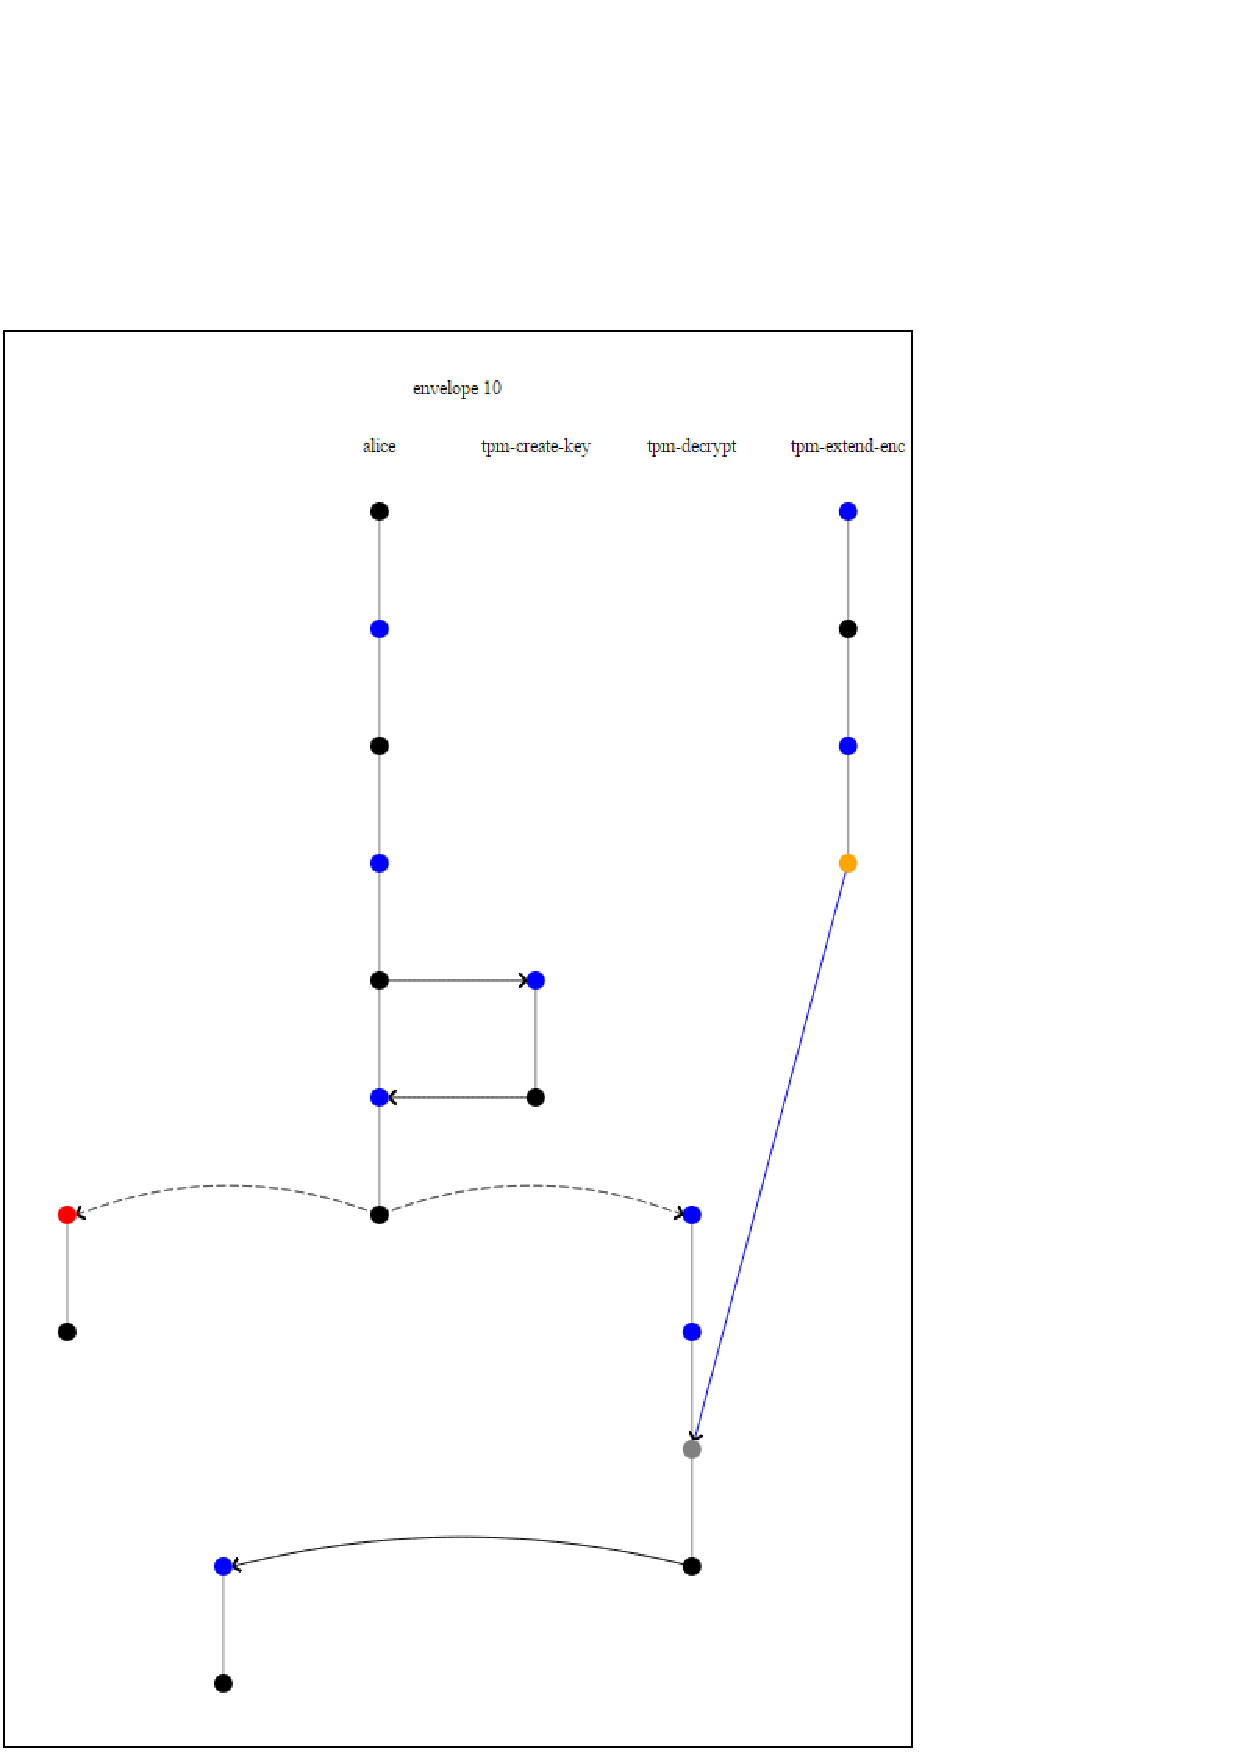
\includegraphics[scale=0.7]{envelope_skel10}
\caption[Graph of a stateful skeleton]{Graph of a stateful skeleton from the Envelope Protocol analysis.  Note the orange node, the gray node, and the blue arrow.}
\label{fig:envelope skel10}
\end{figure}

\ttindex{leadsto} This relationship is noted in a \texttt{leadsto}
field in a \texttt{defskeleton}, and is displayed when graphed as
a blue arrow.  Note that the graphing program will only display a
blue arrow when the two related state events are in distinct strands.
If such a relation is determined between two state events in the same
strand, the tool will note it in the \texttt{defskeleton} output, but
the arrow will not show up in the graph.

\begin{figure}
  \centering\tabcolsep=2em
    \begin{tabular}{cc}%\SelectTips{cm}{}
      \xymatrix@R=8ex@C=.7em{
        &\circ\ar@{~>}[dr]\ar@{~>}[dl]\\ \texttt{tran}&=&\texttt{tran}
      } &
      \xymatrix@R=8ex@C=.7em{
        &\circ\ar@{~>}[dr]\ar@{~>}[dl]\\ \texttt{obsv} & \leftarrow & \texttt{tran}
      }
%\xymatrix@R=2.5ex@C=2em{
%        \tran(\cdot,t)\ar@{~>}[dr]\ar@{->}[dd]\\ &\tran(t,\cdot)
%        \ar@{<~}[dl]^(.3){\mbox{~}}\\ \obsv t\\ }
      \\ (1)& (2)
    \end{tabular}
  \caption[State-respecting semantics]{State-respecting semantics.
    (1) State produced (either from a \texttt{tran} or \texttt{init}
    event) cannot be consumed by two distinct transitions.  (2)
    Observation occurs after the state observed is produced but before
    that state is consumed by a subsequent
    transition.}\label{fig:sequential semantics}
\end{figure}

Two important semantic rules are enforced by the tool regarding state.
First, state produced can only be consumed by a unique transition.  In
other words, state evolves in a linear fashion, and old states are not
available for modification.  Second, when a state is observed, and
that state is also consumed by a transition, the observation must
occur before the transition.  See Figure~\ref{fig:sequential semantics}.

\subsection{Macros for Simplifying Complex Protocols}
\label{sec:macros}

Users will often find, as they try to model more and more complicated
protocols, that models of protocols created by hand are cumbersome to
maintain.  For instance, one might have a particular encrypted message
component referenced in several roles in a model, and the user may
decide they should modify their model of that message.  The user would
normally have to find each instance of the model and update them all:
a repetitive task that would best be handled by computers.

The envelope protocol includes such a feature in a couple of places.
For example, we chose to model TPM register extension using the
\texttt{hash} function symbol, and this modeling choice affects many
protocol roles.

\ttindex{defmacro} \index{macros}
The {\cpsa} tool includes a macro functionality that helps with this
kind of challenge, and the \texttt{envelope.scm} example also serves
as an example of macro use.

To define a macro in a {\cpsa} input file, use the \texttt{defmacro}
keyword in an S-expression.  The \texttt{envelope.scm} file in the
examples directory uses the following two macros:

\begin{verbatim}
;;; Encoding of a PCR extend operation
(defmacro (extend val old)
  (hash val old))

;; This is the refusal token
(defmacro (refuse n pcr v k aik)
  (enc "quote" (extend "refuse" (extend n pcr)) (enc v k) aik))
\end{verbatim}

The first input to the defmacro defines the format that will trigger
the macro.  In this case, the first macro is defined for an
S-expression with keyword \texttt{extend} and two additional inputs,
while the second macro is defined for an S-expression with the keyword
\texttt{refuse} and five additional inputs.

The second input to each defmacro describes what the macro should be
replaced with.  Symbols that exactly match the subsequent symbols in
the first input are interpreted as standing for the inputs when the
macro is used.  So for instance \texttt{(refuse a b c d e)} would be
replaced by

\begin{verbatim}
(enc "quote" (extend "refuse" (extend a b)) (env c d) e)
\end{verbatim}

\noindent
which in turn would be replaced by

\begin{verbatim}
(enc "quote" (hash "refuse" (extend a b)) (env c d) e)
\end{verbatim}

\noindent
\index{macros!nesting} Macros can call on other macros, (as in the
\texttt{refuse} macro example here) but there is a depth limit to the
amount of recursion that this can entail.

\ttindexalt{\^}{(macro splicing)}
\index{macros!splicing} Normally a \texttt{defmacro} will
replace a symbol with a single S-expression, but the \texttt{\^}
(splice) keyword can be used to indicate that a macro should be
replaced with more than one S-expression.

A user might use this feature to replicate a sequence of events or even
the entire variables and trace of a \texttt{defrole}.  For instance:

\begin{verbatim}
(defmacro (handshake n a b)
  (^ (send (enc "hello" a b n (pubk b)))
     (recv (enc "hello-received" a n (pubk a)))))
\end{verbatim}

Note that the pre-processor actually handles the splice keyword as a
separate pre-processing step after macro expansion.  For this reason,
use of \texttt{\^} outside of macros can produce unanticipated behavior.

%%% Local Variables:
%%% mode: latex
%%% TeX-master: "cpsa4manual"
%%% End:
